\begin{mdframed}
    \textbf{La extensión máxima para esta sección es de 6 páginas.}
\end{mdframed}


En esta sección, los resultados obtenidos, como las gráficas o tablas, deben estar respaldados por los datos generados durante la ejecución de sus programas. Es fundamental que, junto con el informe, se adjunten los archivos que contienen dichos datos para permitir su verificación. Además, se debe permitir y especficiar como obtener esos archivos desde una ejecución en otro computador (otra infraestructura para hacer lso experimentos).

\textbf{Es necesario automatizar la generación de las gráficas}, ya que es imprescindible que se pueda confirmar que las visualizaciones presentadas son producto de los datos generados por sus algoritmos.

Agregue gráficas que muestren los resultados de sus experimentos. La cantidad de páginas es limitada, por lo tanto escoja las gráficas más representativas y que muestren de manera clara los resultados obtenidos. Esta elección es parte de lo que se evaluara en la sección de presentación de resultados. Referencie las figuras en el texto, describa lo que se observa en ellas y por qué son relevantes.




\begin{figure}[H]
    \centering
    \begin{minipage}[t]{0.5\textwidth}
        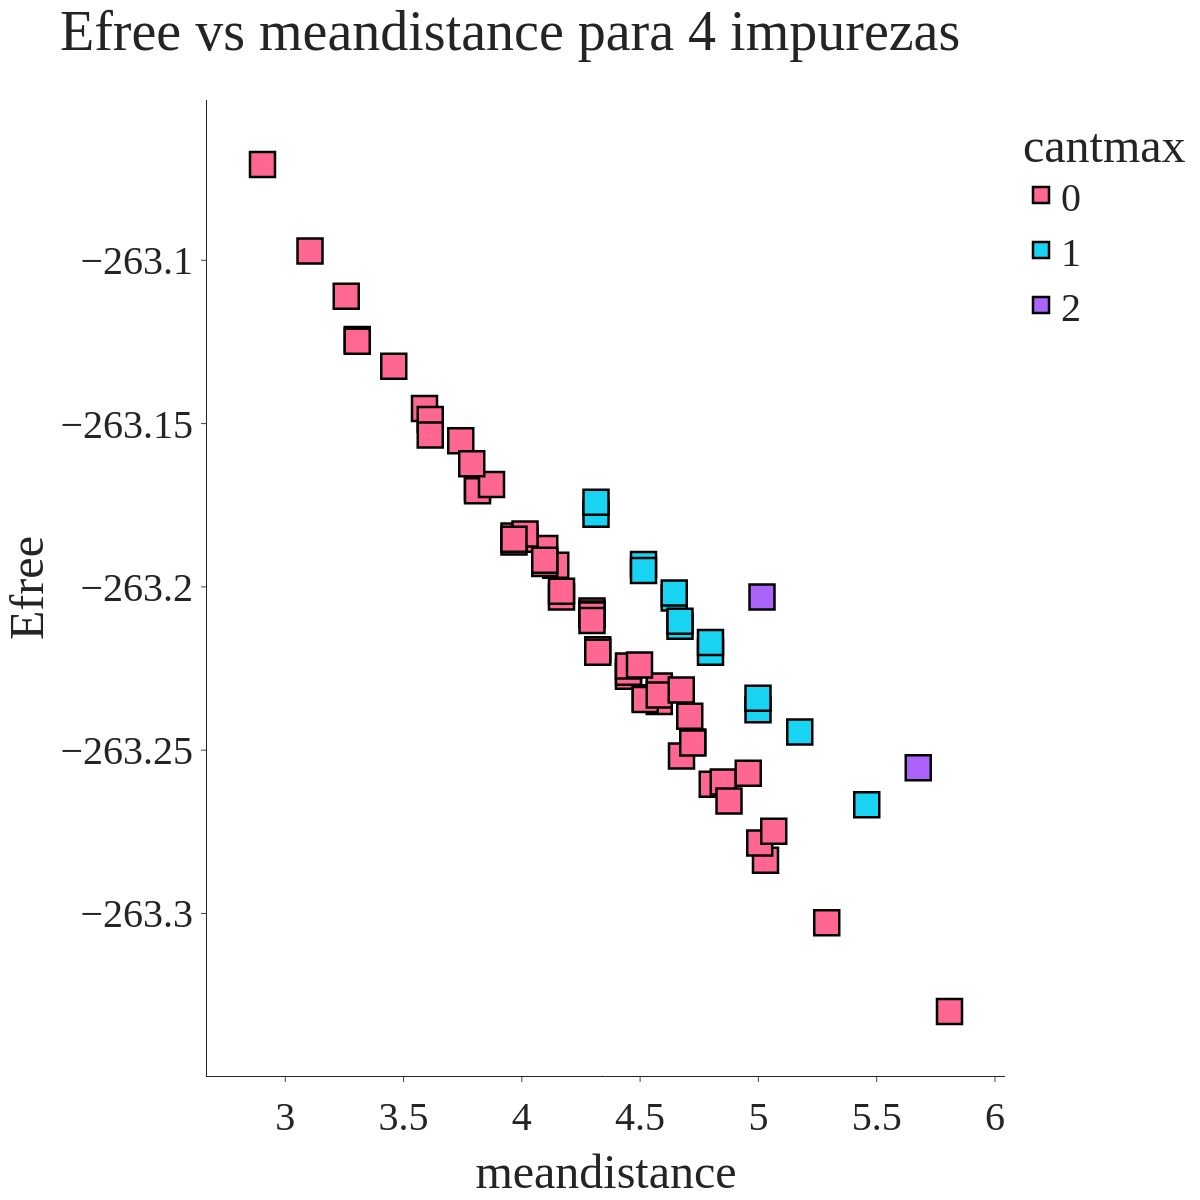
\includegraphics[width=\textwidth]{../code/matrix_multiplication/data/plots/4_impurezas_cantmax_size10.png}
    \end{minipage}%
    \begin{minipage}[t]{0.5\textwidth}
        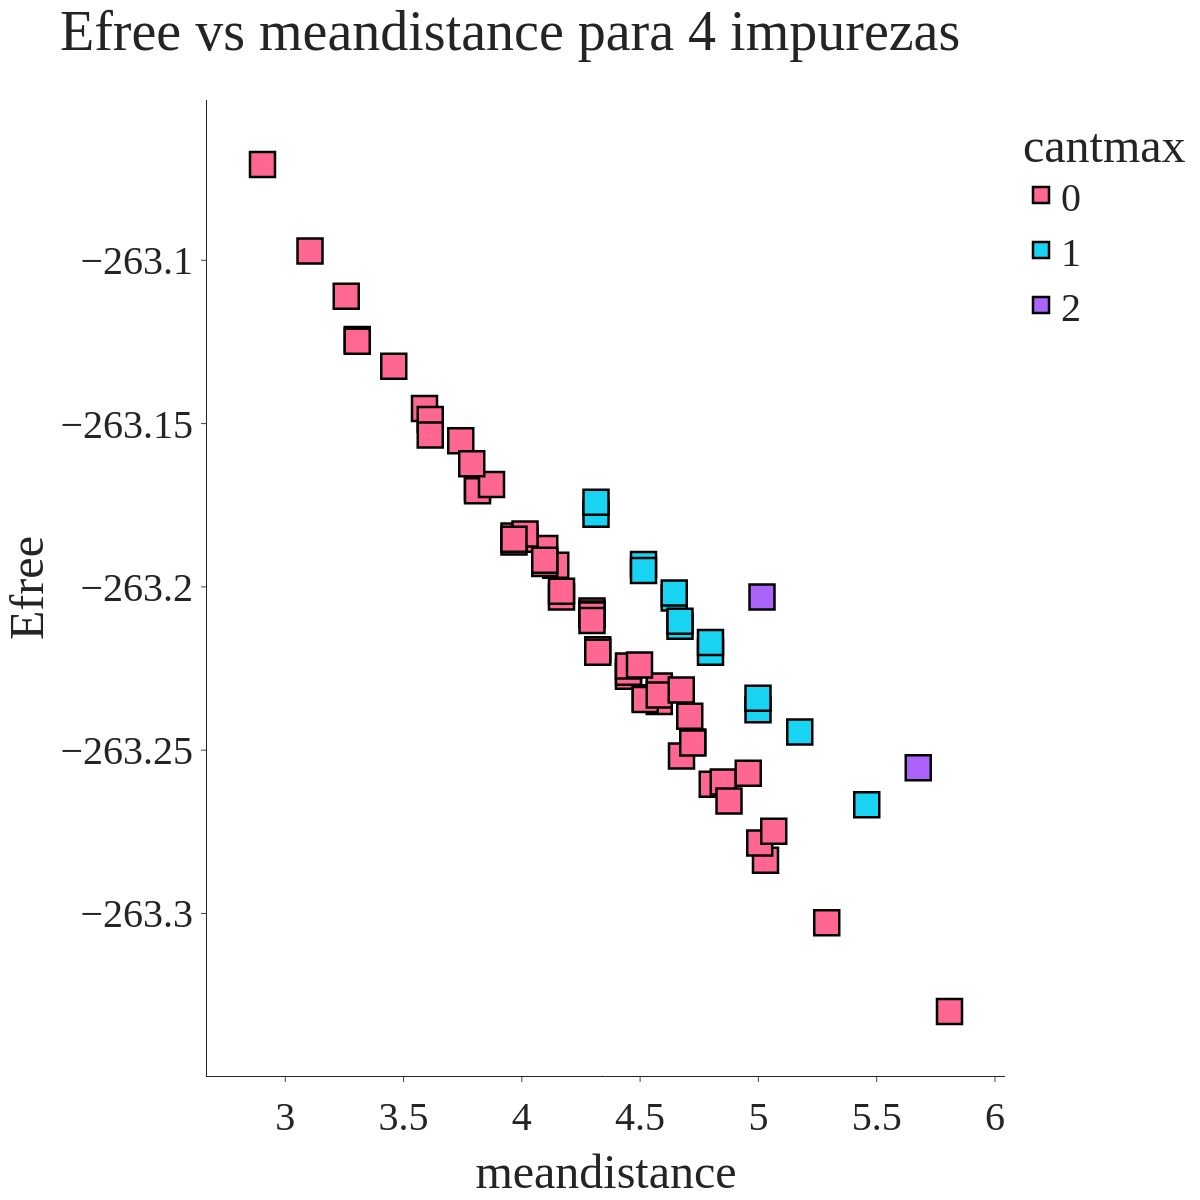
\includegraphics[width=\textwidth]{../code/matrix_multiplication/data/plots/4_impurezas_cantmax_size10.png}
     \end{minipage}%
    \caption{Ejemplo de scatterplot hecho con matplotlib.}
    \label{fig:scatterplot_3}
\end{figure}





\begin{mdframed}
    Recuerde que es imprescindible que se pueda replicar la generación de las gráficas, por lo que usted debe referir a las figuras generadas en `code/matrix\_multiplication/data/plots/` y `code/sorting/data/plots/`.
\end{mdframed}
